%% Springer Nature LaTeX template (sn-jnl.cls) supplied with the submission.
\documentclass[lineno,pdflatex,sn-apa]{sn-jnl}% Math and Physical Sciences Numbered Reference Style

%%%% Standard Packages
\usepackage{graphicx}%
\usepackage{multirow}%
\usepackage{amsmath,amssymb,amsfonts}%
\usepackage{amsthm}%
\usepackage{mathrsfs}%
\usepackage[title]{appendix}%
\usepackage{xcolor}%
\usepackage{textcomp}%
\usepackage{manyfoot}%
\usepackage{booktabs}%
\usepackage{algorithm}%
\usepackage{algorithmicx}%
\usepackage{algpseudocode}%
\usepackage{listings}%
\let\orcidlogo\undefined
\usepackage{orcidlink}%
%%%%

\theoremstyle{thmstyleone}%
\newtheorem{theorem}{Theorem}%
\newtheorem{proposition}[theorem]{Proposition}%

\theoremstyle{thmstyletwo}%
\newtheorem{example}{Example}%
\newtheorem{remark}{Remark}%

\theoremstyle{thmstylethree}%
\newtheorem{definition}{Definition}%

\raggedbottom
\unnumbered


\begin{document}



\title[Feedback timing and residual updating]{Sparse sampling and delayed updating for provisional river nitrate plus nitrite load estimation}



\author*[1,2]{\fnm{Junjie} \sur{Zhang}\,\orcidlink{0009-0004-8821-4018}}\email{junjiezhang2024@shisu.edu.cn}

\affil*[1]{\orgdiv{Shanghai Academy of Global Governance and Area Studies}, \orgname{Shanghai International Studies University}, \orgaddress{\city{Shanghai}, \postcode{201620}, \country{China}}}

\affil[2]{\orgdiv{School of Economics and Finance}, \orgname{Shanghai International Studies University}, \orgaddress{\city{Shanghai}, \postcode{201620}, \country{China}}}


\abstract{Reducing concentration sampling while discharge continues to be observed requires decisions about when to sample and how to use results that arrive after estimates are issued. We retrospectively assessed these decisions using quality screened United States Geological Survey discharge and optical nitrate plus nitrite records from 21 stations during 2019 to 2025, comparing periodic, flow triggered, block deadline and load value schedules under a shared residual correction, a 24 h delay and provisional hourly estimates. Primary event assessments covered 46 high flow episodes at nine temporal stations and 64 episodes at eight additional stations. At 96 annual sampling attempts the temporal mean event absolute relative error was 31.7\% for the historical predictor, 17.7\% for flow triggering and 16.9\% for load value sampling, so returned sample updating produced most of the improvement, whereas the extra advantage of load value over flow triggering was 0.83 percentage points (95\% station interval $-$0.86 to 2.42) and that at the additional stations was 0.09 points ($-$2.52 to 1.99); periodic sampling still gave smaller mean absolute event mass errors than load value sampling in both cohorts. Fixed calendar diagnostics showed that reconstruction choices could reorder schedule rankings, and scoring ablations at fixed realized delays left mean error essentially unchanged, so these post hoc findings support improving the use of returned samples before adding acquisition complexity and selecting a sampling system for the intended error objective within qualified sensor reference windows, while independent laboratory accuracy and complete annual loads would require different data.}



\keywords{optical nitrate; provisional load estimation; sampling design; result delay; residual updating; reference support}



\maketitle



\section{Introduction}\label{sec:introduction}

River nutrient transport varies strongly in time, and continuous optical sensors now resolve that variability at hourly resolution \citep{rode2016,bieroza2023}. A monitoring programme that operates such a sensor holds an unusually rich record of how concentration and discharge move together, and it can draw on that record to estimate transport between the concentration observations it collects. This study evaluates one clearly bounded version of that task. A station already holds several years of high frequency concentration history and continues to observe discharge every hour, concentration sampling is then reduced for a single year, and an analyst issues a provisional concentration estimate at the start of each hour using only the information available at that moment and combines it with the discharge observed during the hour. Issued estimates are never revised, so the endpoint is the quality of the trajectory that an analyst would actually have issued as the year unfolded, rather than the accuracy of a final annual load assembled after every result has returned. The reduced sampling year is a hypothetical monitoring scenario built to keep the comparison controlled, and it does not describe the reporting practice of any particular agency.

Sampling design studies built on high frequency records show that this task has no universal answer. Controlled subsampling of sensor records has been used to test alternative schedules against a dense reference \citep{rode2016,bieroza2023}, and regular sampling has remained competitive with dynamic schedules in river nitrate monitoring \citep{reynolds2016}. Evaluations of load estimation show that accuracy depends on the constituent, the station, the sampling design and the estimator \citep{lee2016,lee2019}. The relationship between concentration and discharge, and the degree to which transport concentrates in short intervals, explain why the same schedule can perform differently across rivers \citep{bieroza2018,moatar2007}. A complex acquisition rule therefore has to add information beyond a credible periodic or flow based schedule, and it has to do so without merely reacting to hydrological variation.

How observations are used is equally consequential. Regression methods such as LOADEST and weighted regressions on time, discharge and season reconstruct concentrations between measurements \citep{runkel2004,hirsch2010}, and residual aware extensions such as WRTDS-K exploit serial correlation to improve that reconstruction \citep{zhang2019}. A retrospective estimate may use observations on both sides of a gap, whereas a provisional estimate can use only results that have already arrived. Even inside that boundary, residual corrections retain information for different lengths of time: pooling many older residuals can stabilise an estimate while preserving a correction that no longer describes the current event. Acquisition rules can be compared fairly only when they share one updater and one information clock, because a common updater equalises access to information but leaves open whether that information is used well.

Responsive sampling and prediction assisted monitoring already have substantial precedents. Urban runoff sampling has been adjusted with environmental information \citep{wong2016}, historical hydrological records have supported forecasts that guide water quality sampling \citep{wilson2026}, and sparse designs have identified informative measurement times from recurring patterns \citep{manohar2018,binmamoon2025}. These methods answer related but distinct questions. An advance calendar, an online selection rule and a retrospective load estimator are not interchangeable when their information boundaries differ, and a comparison across them cannot isolate the contribution of the acquisition rule itself. For the monitoring task studied here, the informative competitors are simple schedules coupled to defensible online corrections, including a schedule that samples only when a block quota would otherwise expire, and a historical predictor that receives no new concentration at all.

Two further distinctions shape the design of such a comparison. The first concerns delay. A rule can account for the return delay of its own samples and for samples that are already awaiting analysis, yet these mechanisms require separate tests: changing the real delay changes the information available to every estimator, whereas changing the delay assumed by the acquisition score leaves actual availability untouched, and a pending result correction can only act when a previous sample is still outstanding at a decision. The second concerns the acquisition objective. A variance reduction score for future residual load is a natural heuristic in the spirit of Bayesian experimental design \citep{chaloner1995}, but its surrogate target need not coincide with the event relative error that a monitoring programme reports.

Three research questions follow, and each is answered with the same quality screened United States Geological Survey record of discharge and sensor nitrate plus nitrite, expressed as nitrogen, from 21 stations during 2019 to 2025 \citep{usgs2026}, which supplies a shared observed window reference rather than independent laboratory truth or a complete annual load \citep{pellerin2013}. First, relative to a historical predictor that receives no new concentration, how much do sparse observations combined with residual updating improve event load error? Second, under the same budget, the same information availability and the same updating rule, does a complex sampling rule add a stable improvement over periodic or flow triggered sampling? Third, how does that comparison depend on the delay before results return, on how residual memory is defined, and on the error objective used for the assessment? Complete systems are compared under one shared output rule and one information clock, the pure block deadline schedule and the historical predictor separate acquisition from updating, fixed calendar diagnostics vary updating family, memory and age origin, fixed real delay ablations isolate the delay terms, and both relative and absolute mass errors are reported so that the objective dependence of the ranking becomes visible.

\section{Materials and methods}\label{sec:materialsandmethod}

\subsection{Study task and information clock}

The study evaluates a single year in which a monitoring station reduces its concentration observations while discharge continues to be recorded every hour. The station already operates a high frequency concentration sensor, so the assessment asks what a reduced concentration programme would have delivered on top of the historical record that the sensor produced. An analyst issues a provisional concentration estimate at the start of each hour using only the information then available, combines that estimate with the discharge observed during the hour, and accumulates transport. Issued estimates are never revised, and cumulative estimates over qualifying high flow episodes form the primary endpoint. The endpoint therefore scores the trajectory that an analyst would actually have issued, rather than a retrospective reconstruction assembled after all results have arrived. Fig. 1 illustrates the four events that the replay keeps separate: collection, result arrival, incorporation into an estimate, and evaluation of the issued trajectory.

Each replay year uses the three preceding calendar years of the same station and requires at least two of them to contain 1,000 qualified exact hour pairs of discharge and concentration. At hour $t$, a policy can access its permitted historical data, calendar variables, discharge observed through $t$, and any purchased concentration that has already returned. The replay receives results that are due, issues the hourly estimate, and then decides whether to purchase a new sample. A purchase at time $s$ returns at time $a=s+d$ and reveals the qualified concentration at the exact collection timestamp. Unpurchased concentrations and future label availability remain hidden, and failed attempts consume the same nominal budget while becoming identifiable only at their scheduled return. Archived discharge enters the replay as a finalized record, so service outages and real time revisions are outside the scope of the simulation.

\subsection{Records, reference support and load units}

Data preparation uses United States Geological Survey discharge parameter 00060 and optical nitrate plus nitrite parameter 99133 for 2019 to 2025. Of 33 candidate stations, 22 had documented colocated discharge and ultraviolet concentration metadata, and one of these lacked usable discharge, which leaves 21 stations with working records. Instrument documentation identifies SUNA, ISUS or Nitratax measurements with UV method codes 012 to 016. Only approved, finite and nonnegative values without estimated or censored qualifiers enter the concentration reference. These screens reduce avoidable measurement uncertainty, and they leave the residual possibility of shared sensor bias that is addressed in the Discussion \citep{wagner2006,pellerin2013}.

Source discharge is reported in cubic feet per second and is converted to $Q$ in cubic metres per second with the factor 0.028316846592. Concentration $c$ is expressed in mg N L$^{-1}$. A complete UTC reference hour requires qualified pairs at its start and at 15, 30 and 45 min. Its reference mass and water volume are

\begin{align}
L_t &= 10^{-3}\sum_{j=0}^{3}Q_{t+15j}c_{t+15j}(900),\\
V_t &= \sum_{j=0}^{3}Q_{t+15j}(900).
\end{align}

Here $V_t$ is in m$^{3}$ and the factor $10^{-3}$ converts mg L$^{-1}$ multiplied by m$^{3}$ into kg. Reference concentration is never interpolated and missing hours are never expanded into annual transport. A prediction uses the issued concentration at the start of the hour multiplied by the realized volume within that hour, $\widehat L_t=10^{-3}\widehat c_t V_t$, so the endpoint scores concentration reconstruction against a common observed volume instead of forecasting future discharge. Online Resource 1 provides an independent numerical unit example and the complete preparation lineage.

A target year enters the assessment when at least 50\% of its calendar hours are complete reference hours. The experiment uses original stations in 2023 and 2024 for configuration development, additional stations in the same years for assessment of the policy specification, and eligible 2025 records for the temporal assessment. Temporal and additional station strata are reported together so that the two generalization questions remain distinct \citep{roberts2017}.

Reference support is described in both time and water volume. Complete reference water volume is compared first with the volume of all finite and nonnegative quarter hour grid discharge readings, each weighted by 900 s independently of concentration availability and including estimated or provisional discharge, and second with a denominator that retains only quality qualified discharge. Neither denominator recovers runoff that was never observed. Within the observed reference support the assessment quantifies the load fraction at or above the historical discharge 90th percentile and the fraction carried by the largest 10\% of hourly masses; the second quantity is an explanatory target year diagnostic that no analyst could compute before monitoring. For eligible events, the reference mass transported before the event start plus 24 or 72 h measures how much transport precedes a hypothetical sample taken at event onset. That quantity describes time coverage rather than an unavoidable error bound or a guaranteed sampling opportunity.

\subsection{Historical predictor and comparison schedules}

Every station, year and seed combination shares one random forest concentration predictor trained on at most 12,000 qualified historical pairs with 64 trees, a maximum depth of 12 and a minimum leaf size of 16 \citep{breiman2001}. Inputs are log scaled discharge, its lags and changes at 1, 6, 24 and 72 h, a 24 span exponentially weighted mean, a discharge missingness indicator, and annual sine and cosine terms. The historical median discharge $Q_*$ supplies the scale. Missing discharge is carried forward for at most 24 h and then replaced by the historical median, and no backward interpolation is used. A forward prediction into the latest eligible historical year, trained only on earlier years, supplies the initial residual scale. Discharge normalisation in that calibration uses the permitted historical window, which makes it forward label calibration rather than a fully nested feature scaling evaluation.

The core comparison contains periodic, flow triggered, pure block deadline and delayed load value schedules. All operate at 24, 48 or 96 attempted samples per calendar year on a 6 h candidate grid with a minimum separation of 24 h and one attempt in each approximately equal calendar block. Periodic phases are 0.25, 0.50 and 0.75 for seeds 41, 73 and 109. The block deadline schedule purchases only at the last permissible candidate in a block and consults neither flow nor uncertainty nor concentration. Flow triggering scores scaled discharge multiplied by one plus its positive 6 h log change. Flow and value scores are compared with a fixed historical context quantile of 0.85 under the current state, and a block deadline fallback guarantees that the quota is completed. The deadline baseline therefore carries the same scheduling obligation without the active score, while failed purchases remain budgeted attempts and results that return after the end of the year cannot alter the scored trajectory. Historical QR and D optimal calendars, randomised schedules and discharge weighted uncertainty are reported in Online Resource 3 as additional schedules from the same experiment.

\subsection{Online reconstruction and fixed calendar components}

The core systems issue predictions from the latest successfully returned residual with a fixed 168 h exponential time constant and an arrival time origin:

\begin{equation}
\widehat c_t=\max\{0,c_0(x_t)+[c_s-c_0(x_s)]\exp[-(t-a)/168]\},\qquad a\le t.
\end{equation}

Before any successful result the system issues the historical predictor. The latest residual is defined by the latest arrival rather than the most recent attempt. Every system issues this output, and each purchase saves the prediction that the system actually made, so the reconstruction rule and the acquisition state are separate and declared components of the load value system. The value system additionally maintains an internal random feature state, constructed as in \citep{rahimi2007}, that drives acquisition, and its innovation scale update uses the saved output prediction. The three simple schedules share the same output rule, the same permitted data and the same collection constraints, and a historical predictor that receives no purchased concentration serves as an explicit comparator.

Fixed calendar components answer a separate question. On development station years at a budget of 96 samples and seed 41, three simple calendars are held constant while the reconstruction half life, the origin of the information age and the update family vary. The half lives are 168 ln 2 h, 720 h and 2160 h, and the first corresponds exactly to the 168 h exponential time constant. Ageing begins either at collection or at arrival, and the update families are the pooled regularised random feature residual model and the latest residual correction. Innovation scale is held fixed in this diagnostic. The matched values are nominal half lives: in the pooled model they discount data precision and its information vector, whereas in the latest correction they attenuate residual amplitude directly, and the pooled model also retains prior precision. Equal nominal half lives therefore need not imply equal predictive memory or equal impulse responses, and a change of update family changes pooling and shrinkage as well as the representation of the residual.

The value score is a model conditional variance reduction heuristic whose information gain concerns the internal acquisition surrogate rather than a calculated variance reduction of the latest residual output. With collection time features $z_t$, projected pre arrival covariance $P^-$, an effective innovation scale $R_t$, discount $\lambda$, an assumed scoring delay $d_s$ and a load functional $v_t$ over 72 h that begins at the assumed arrival and is truncated at the end of the year, the score is

\begin{equation}
S_t=\frac{(v_t^{\mathsf T}P^-z_t)^2}{R_t/\lambda^{d_s}+z_t^{\mathsf T}P^-z_t}.
\end{equation}

Both $P^-$ and $v_t$ are built with $d_s$, while actual availability still follows $a=s+d$. Future discharge inside $v_t$ persists at the currently available discharge and only calendar terms are known in advance. Pending observations contribute expected information but never an unrevealed concentration. Online Resource 1 gives the state update and the original settings. The score carries squared load units under a linear Gaussian surrogate, its covariance is not calibrated reality, and no optimality or regret guarantee is claimed. It targets absolute future residual load uncertainty, whereas the primary endpoint weights event relative errors equally, and that difference is measured rather than assumed away.

\subsection{Mechanism and historical state diagnostics}

At a real delay of 24 h, results that are due arrive before the next permissible purchase, so no earlier purchase can still be pending at an eligible decision and queue awareness is inactive in the main scenario. The mechanism tests hold actual result return times fixed and change only the delay assumed by the score, or, at a real delay of 72 h, omit the expected information from pending purchases. They therefore compare complete systems under one actual information clock. Candidate traces record pending counts, score triggered samples and quota fallback, which prevents an implemented but inactive mechanism from being read as a demonstrated benefit.

Historical residual persistence is estimated from forward historical predictions with exactly lagged pairs and continuously qualified intermediate support, and training in sample residuals are not used. Target period bias and shifts are reported as explanatory diagnostics. A separate candidate information diagnostic uses development stations in 2023 and 2024, seed 41 and the budget 96 periodic calendar, and nominates the sole candidate of each month at 12:00 UTC on the 15th without replacement. At a real delay of 24 h the diagnostic compares predictions with and without that additional sample over the 72 h that follow its arrival, while keeping the subsequent purchase calendar and its saved innovation weights fixed. The two latest residual trajectories coincide again after the next successful scheduled return. Future reference values enter only the declared evaluation screens, which are 95\% coverage and positive reference mass, and the realized error calculation. The added sample is a diagnostic rather than a competing policy at an equal budget, so it measures the alignment between a prospective score and realized information utility without estimating the environmental effect of deploying a policy. Event process illustrations use the maximum improvement, the maximum deterioration and the median difference in load value versus flow trigger event absolute relative error at a budget of 96 samples and seed 41, and the complete station outcomes remain visible alongside them.

\subsection{Endpoints and uncertainty}

High flow episodes reach or exceed the historical discharge 90th percentile, may join at most 24 observed hours below that threshold, and last at least 12 h. Missing discharge splits an episode. An event is scored only when at least 95\% of its reference hours are complete and its boundaries are determinate, which requires no missing discharge in the preceding and following 24 h and no crossing of a calendar year edge. Retained and excluded episodes are compared for peak discharge, duration, season and the position of missing reference hours, and excluded concentration mass is never treated as observed truth.

The primary endpoint is the mean event absolute relative load error over common valid hours. Event errors are averaged within station, year and seed, then across seeds, then across available years within a station, and finally with equal weight across stations. A sensitivity requires at least three eligible events per station year. Secondary outcomes cover signed and absolute event load differences in kg N, observed window bias, hourly load error, concentration error and the proportion of events within analyst selected absolute relative error thresholds of 10\% or 20\%. Those thresholds are illustrative accuracy scenarios rather than regulatory standards, and whole window outcomes retain stations without qualifying events. Nominal sample counts are not monetary costs.

Paired differences use the same station, year, seed and reference support, and positive values denote baseline error minus candidate error. Pointwise 95\% percentile intervals use 10,000 station resamples with seed 271828, and coarse HUC4 group resampling and leave one group out results probe geographical influence. HUC4 membership is not proof of independence, and events, hours and seeds are nested observations rather than additional independent catchments. No multivariable applicability model is fitted to nine temporal stations.

\subsection{Analysis status and scope}

All comparisons reported here were executed after the evaluation records had been inspected, so they are post hoc analyses of an inspected record set rather than an independent validation of a pre registered policy. The settings of the earlier experiment, which supplies the pooled output comparator, were recorded before the policy outcomes of those assessments were inspected, and Online Resource 3 lists which components were fixed before which results were examined. The 24 h main delay and the 6 h and 72 h variants are experimental information constraints and not claims about laboratory turnaround norms, sample holding times or data review delays. The analyses describe the qualified sensor reference, the declared information clock and the observed support of these records; extending them to laboratory accuracy, indefinite sparse operation or unmonitored rivers would require different data.

\subsection{Computational verification}

Every numerical result comes from archived observations and executable code. Separate implementations checked chronology, budgets, units, event endpoints and aggregation, and the figures were drawn deterministically from the recorded results without generated visual data. These computational checks support the scientific review and accountability of the author.

\section{Results}\label{sec:results}

\subsection{Transport concentration and the support of the reference}

The 21 station working dataset contains 1,288,728 hourly records and 748,679 complete reference hours across 2019 to 2025. Historical qualification and target year support leave 13 station years for the temporal assessment and 16 station years at eight additional stations for the 2023 and 2024 assessment. The primary event endpoint uses nine temporal stations with 46 eligible episodes and eight additional stations with 64 episodes in 14 station years (Table 1; Fig. 1). These events belong to five and six HUC4 groups respectively, and four temporal stations had no eligible positive load event while remaining in whole window assessments. Quality and boundary screening retained 46 of 147 defined temporal events and 64 of 161 additional station events (Fig. S1), so the event population is narrower than all high flow transport. Station identifiers and the number of qualified working records are listed in Table S1.

\begin{table}[htbp]
\caption{Evaluation support after data qualification and event screening}\label{tab:1}
\footnotesize
\setlength{\tabcolsep}{2pt}
\begin{tabular}{@{}lccccc@{}}
\toprule
\shortstack{Assessment\\records} & \shortstack{Data sites /\\site years} & \shortstack{Primary sites\\/ site years} & \shortstack{Eligible /\\defined events} & \shortstack{Primary HUC4\\groups} & \shortstack{Reference\\water median\\(\%)}\\
\midrule
Development 2023 to 2024 & 7 / 14 & 7 / 13 & 36 / 65 & 5 & 91.48\\
Additional stations 2023 to 2024 & 8 / 16 & 8 / 14 & 64 / 161 & 6 & 94.58\\
Temporal 2025 & 13 / 13 & 9 / 9 & 46 / 147 & 5 & 94.39\\
\botrule
\end{tabular}
\end{table}

Water support is the median across data eligible station years, computed as complete reference volume divided by the volume of all observed finite and nonnegative quarter hour grid discharge, and events are eligible events over defined events. Event endpoints require at least one eligible episode with positive mass. HUC4 groups describe geography rather than independent replication, and the development and temporal records can involve the same stations.

\begin{figure}[htbp]
\centering
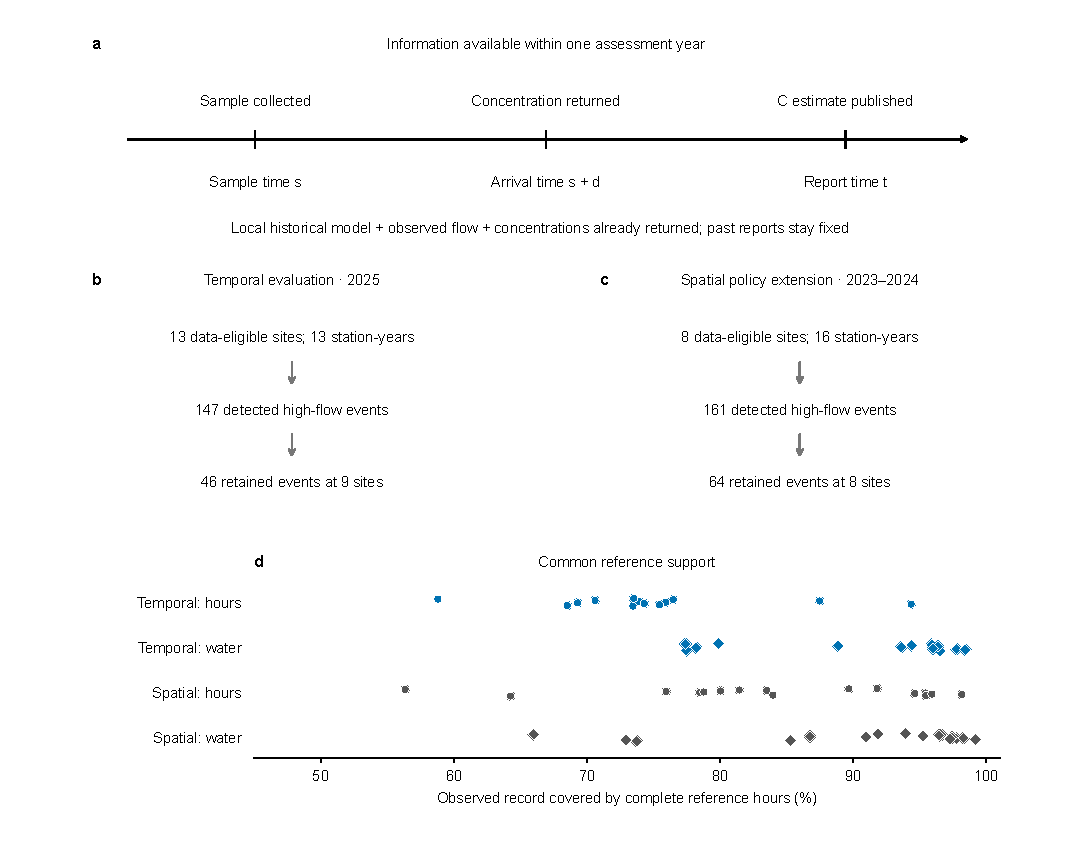
\includegraphics[width=\textwidth]{figures/Fig1.pdf}

\caption{Information clocks, evaluation cohorts and observed reference support. (a) Schematic information sequence: a concentration collected at s becomes available at s + d, the estimate issued at the start of hour t uses only information available at that moment, and the estimate is never revised. Hourly transport accumulates as flow is observed during the hour, and its completed integral is unknown at the start of the hour. The schematic illustrates the design and is not an observed event. (b, c) Data eligible station years together with detected and retained events for the temporal assessment and the spatial policy extension, where each site supplies its own local concentration history. Retention requires the specified complete hour coverage and observable flow boundaries. (d) Each point is one data eligible station year, 13 temporal and 16 spatial. Hours are complete reference hours divided by calendar hours. Water is the volume in complete reference hours divided by all available numeric nonnegative quarter grid flow volume, including provisional and estimated flow, which is observed flow volume and not unobserved runoff. Seeds add computation rather than environmental replication, and no missing transport is imputed.}
\label{fig:1}
\end{figure}

Transport concentrates in relatively few observed hours (Fig. 2). Across temporal station years, the largest 10\% of complete hourly masses carry a median 42.37\% of reference transport and hours above the historical discharge 90th percentile carry a median 53.23\%. The corresponding additional station medians are 49.04\% and 43.26\%. These fractions describe where the recorded transport occurred, and the classification by largest hourly mass is not available as a selection input.

Reference support is also uneven. Complete reference water volume represents a median 94.39\% of temporal observed discharge volume, with a station year range of 77.42\% to 98.43\% and a pooled ratio of 90.89\%, and the additional station values are 94.58\% and 90.48\%. These ratios use observed native discharge as the support denominator and they do not recover missing concentration mass. Retained temporal events have a median duration of 58 h and a median peak discharge of 243.52 m$^{3}$ s$^{-1}$, compared with 43 h and 125.16 m$^{3}$ s$^{-1}$ among excluded events, and the reference is complete at the discharge peak in 45 of 46 retained episodes and 75 of 101 excluded episodes. Seasonal composition differs as well: retained events include 3 winter, 18 spring, 23 summer and 2 autumn episodes, while excluded events include 10, 28, 44 and 19. Because these comparisons pool stations, they describe the selection that the coverage rules produce rather than a general within river mechanism (Fig. S1; Online Resource 1).

Information timing constrains the provisional task without setting a fixed error floor. For a hypothetical sample collected at event onset, the median eligible temporal event has already transported 42.50\% of its reference mass before a 24 h return and 100\% before a 72 h return, while the mass weighted fractions are 13.36\% and 35.06\%. Additional station medians are 43.45\% and 100\%, with mass weighted fractions of 25.18\% and 61.01\%. Long events dominate the mass weighted summaries, so the typical event and the mass weighted view answer different questions, and a historical model or a sample collected before onset can still supply information during these intervals.

Forward historical residuals show substantial and heterogeneous persistence. Across the 13 temporal station years, median lag correlations are 0.963, 0.859, 0.694 and 0.468 at 6, 24, 72 and 168 h with continuously qualified support, and the 168 h correlation ranges from $-$0.025 to 0.872 (Fig. S2). These residuals come from forward predictions and never from training in sample errors, and they support residual updating without identifying a single useful correction lifetime. The historical predictor reaches a temporal event error of 31.74\% against 19.07\% at the additional stations, so the two cohorts differ in how much error a returned sample can remove (Fig. S2). These forward transfer differences describe the evaluation records and are not isolated evidence of concept drift.

\begin{figure}[htbp]
\centering
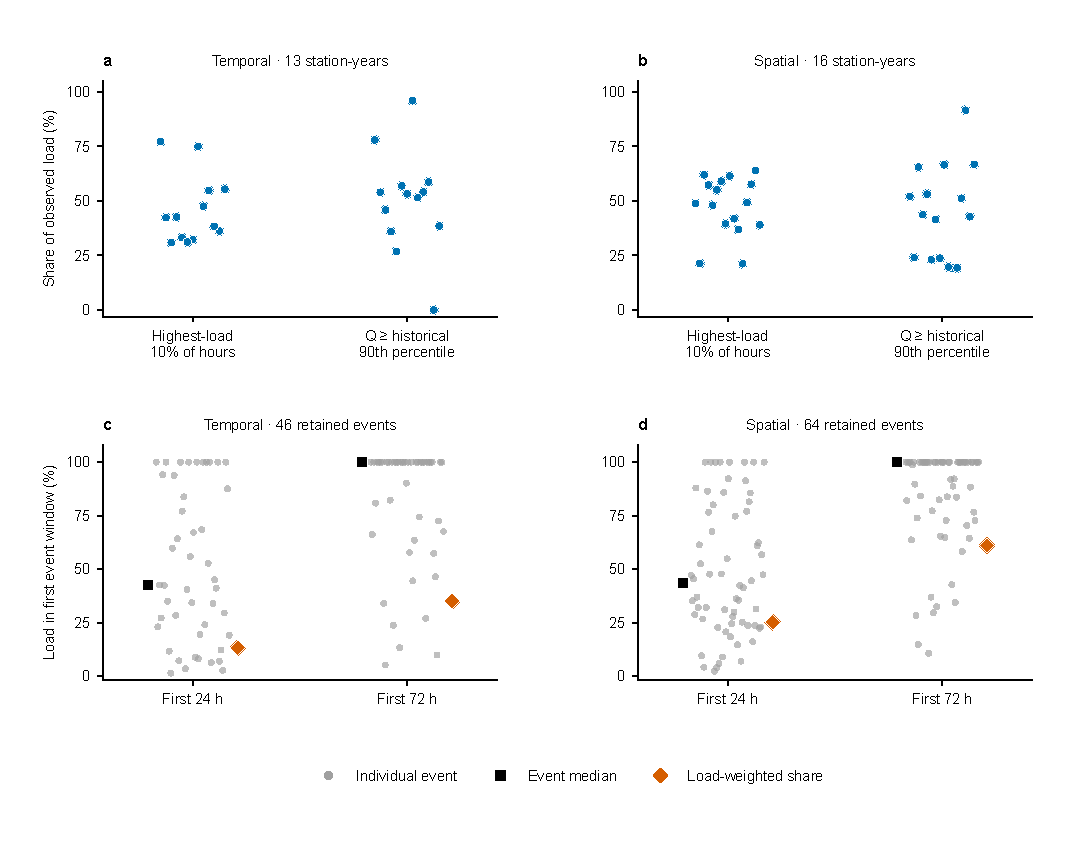
\includegraphics[width=\textwidth]{figures/Fig2.pdf}

\caption{Observed transport concentrates in time, and the timing summary depends on its weighting. (a, b) Each point is a data eligible station year: the fraction of complete hour reference load in the highest load 10\% of complete hours, and in complete hours whose exact hour flow reaches the preceding three year flow 90th percentile. The top hour count is ceil(0.10 $\times$ complete hours). (c, d) Fractions of retained event reference load transported during the first 24 or 72 h after event onset. Grey dots are individual events, black squares are unweighted event medians, and vermilion diamonds weight events by observed reference load. A short event can reach 100\% while contributing little to the load weighted total. These fixed window quantities describe a hypothetical sample at event onset rather than the first result arrival of a policy, and they are not a lower bound on estimation error. Only retained events with positive reference load are included, which are 46 temporal events at nine sites and 64 spatial events at eight sites, and event points are nested within sites. All quantities are restricted to observed reference support.}
\label{fig:2}
\end{figure}

\subsection{Complete systems with a common output rule}

All four systems complete their nominal attempt budgets while respecting result availability, block quotas and minimum spacing, and their event errors appear with the zero label comparator in Table 2 and Fig. 3. At temporal budgets of 24, 48 and 96 samples, the delayed load value system reaches 22.8\%, 21.2\% and 16.9\% mean absolute relative error; periodic sampling gives 25.8\%, 22.2\% and 20.7\%; flow triggering gives 23.9\%, 22.1\% and 17.7\%; and pure deadline sampling gives 25.5\%, 24.3\% and 19.4\%. Two layers of improvement have to be kept apart. Relative to the unchanged historical predictor at 31.7\%, returned sample updating improves the endpoint substantially: load value sampling gains a paired mean of 14.87 percentage points, with a pointwise station resampling interval of 8.61 to 21.12 points, and improves all nine temporal stations, while flow triggered sampling reaches 17.7\% and so improves the same endpoint by 14.0 points. The second layer, the extra value that the complex rule adds on top of the simple hydrological trigger, is much smaller and is quantified next.

\begin{table}[htbp]
\caption{Complete system event mean absolute relative error (\%)}\label{tab:2}
\footnotesize
\setlength{\tabcolsep}{2pt}
\begin{tabular}{@{}lcccccc@{}}
\toprule
& \multicolumn{3}{c}{Temporal} & \multicolumn{3}{c}{Additional} \\
\cmidrule(lr){2-4}\cmidrule(lr){5-7}
System & 24 & 48 & 96 & 24 & 48 & 96 \\
\midrule
Periodic & 25.75 & 22.18 & 20.68 & 18.52 & 17.54 & 15.59\\
Flow trigger & 23.86 & 22.13 & 17.70 & 17.42 & 16.09 & 14.64\\
Block deadline & 25.54 & 24.29 & 19.41 & 21.94 & 20.16 & 17.49\\
Load value & 22.81 & 21.19 & 16.87 & 18.45 & 16.74 & 14.55\\
Historical predictor & 31.74 & 31.74 & 31.74 & 19.07 & 19.07 & 19.07\\
\botrule
\end{tabular}
\end{table}

Budgets are annual attempted samples. Every sampled system uses the latest returned residual with a 168 h exponential time constant from arrival and a 24 h actual delay, and failed attempts count against the budget. Events are averaged within station, year and seed, then across seeds, then across years within station, and finally with equal weight across stations. The historical predictor purchases nothing and appears at every budget for comparison.

The additional value of the complex trigger is much smaller. At a temporal budget of 96 samples, load value error is 0.83 percentage points below flow triggering with a station interval of $-$0.86 to 2.42 points, and six of nine stations improve. The difference from periodic sampling is 3.81 points ($-$0.01 to 7.96) with seven improving stations, and the difference from pure deadline sampling is 2.54 points (0.99 to 4.17) with seven improving stations. Scheduling before quota expiry therefore adds information in this setting, while the data do not establish a stable advantage over a simple hydrological trigger. Coarse HUC4 resampling includes zero for the flow comparison ($-$0.68 to 2.30 points), and the station level pattern appears in Fig. S3. Table S2 in Online Resource 2 lists every paired interval, including all three budgets.

At the additional stations, load value errors are 18.5\%, 16.7\% and 14.6\% against 17.4\%, 16.1\% and 14.6\% for flow triggering. At a budget of 96 samples load value error is 0.09 points lower than flow triggering, so the paired difference, flow minus value, is 0.09 points with a station interval of $-$2.52 to 1.99, and five of eight stations improve. The difference from the historical predictor is 4.52 points ($-$2.36 to 10.97) with five improving stations, and the difference from deadline sampling is 2.95 points (0.93 to 5.67) with seven improving stations. Timely updating therefore helps on average at these stations, and the cohort still contains stations whose already adequate historical predictor was harmed by a new correction. Universal benefit from purchasing or adaptively selecting labels is not implied by these results.

\begin{figure}[htbp]
\centering
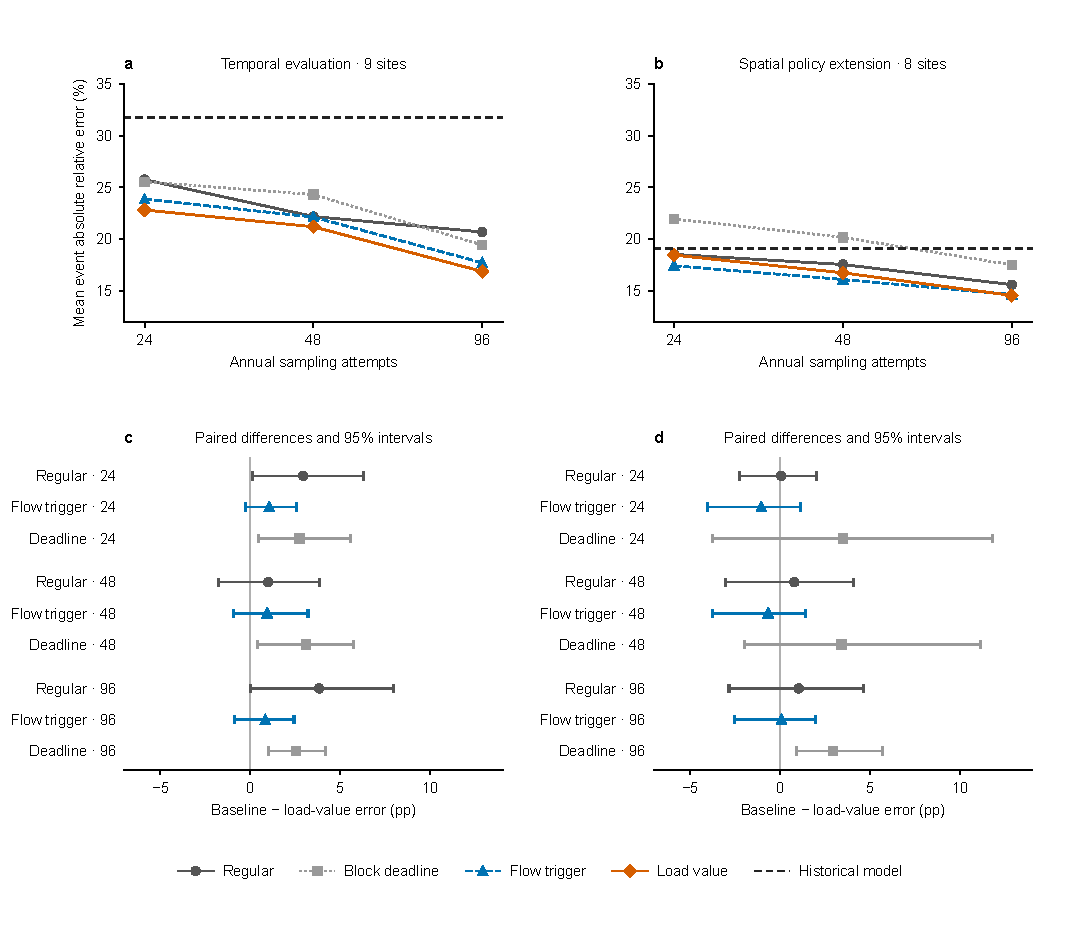
\includegraphics[width=\textwidth]{figures/Fig3.pdf}

\caption{Complete sampling systems under one online reconstruction rule. (a, b) Mean station level event absolute relative error for the four policies at 24, 48 and 96 annual sampling attempts with the actual result return delay fixed at 24 h. All systems use the latest returned residual with arrival origin exponential decay and a 168 h time constant. The horizontal historical predictor line receives no new labels and is charged none of the plotted sample budgets. The temporal assessment contains nine event eligible sites and 46 retained events, and the spatial policy extension contains eight sites and 64 retained events across 2023 and 2024, where each site provides its own historical calibration data. Seed and year averaging precede equal site averaging. (c, d) Paired station mean differences, baseline minus load value, with 95\% station bootstrap intervals. Positive values favour load value, and intervals that cross zero indicate uncertain direction at this sampling level. Differences are percentage points of relative event error rather than kilograms of nitrogen. The event endpoint gives events equal weight within a site.}
\label{fig:3}
\end{figure}

\subsection{Sampling system rankings depend on the assessment objective}

The choice of error objective decides which sampling system ranks first (Table 3). At a temporal budget of 96 samples, load value sampling reduces event mean absolute relative error relative to periodic sampling, while periodic sampling achieves the smaller equal station mean absolute event mass error of 47.53 thousand kg N against 51.80 thousand kg N. The paired difference, periodic minus load value, is $-$4.27 thousand kg N with a pointwise station interval of $-$26.16 to 10.99 thousand kg N, so the point estimate favours periodic sampling while the interval includes zero. At the additional stations the corresponding mass errors are 24.55 and 25.88 thousand kg N, a paired difference of $-$1.32 thousand kg N ($-$12.30 to 5.56 thousand kg N). Against flow triggering the mass error favours load value sampling, by 7.74 thousand kg N in the temporal cohort ($-$1.74 to 22.85 thousand kg N) and by 0.71 thousand kg N at the additional stations ($-$1.35 to 2.72 thousand kg N). Whole window hourly load errors are nearly equal at the largest budget. Reducing event relative error and reducing event mass error therefore do not call for the same sampling choice, and with nine and eight stations the intervals remain wide in both directions. Under the illustrative 20\% event error scenario, the load value system reaches the threshold for an equal station mean 76.46\% of temporal events and 80.07\% of additional station events, against 72.54\% and 79.14\% for flow triggering. Temporal events with error above 50\% comprise 6.61\% for load value and 6.00\% for flow. These summaries are accuracy scenarios rather than regulatory pass rates, and they cannot be merged into a single claim of dominance.

\begin{table}[htbp]
\caption{Error magnitude and illustrative accuracy scenarios at a budget of 96 samples}\label{tab:3}
\footnotesize
\setlength{\tabcolsep}{2pt}
\begin{tabular}{@{}lccccc@{}}
\toprule
& & \multicolumn{2}{c}{Mass error ($10^{3}$ kg N)} & \multicolumn{2}{c}{Event share (\%)} \\
\cmidrule(lr){3-4}\cmidrule(lr){5-6}
Cohort & System & Signed & Absolute & Within 20\% & Above 50\% \\
\midrule
Temporal & Periodic & $-$5.95 & 47.53 & 69.53 & 9.61\\
Temporal & Flow trigger & +13.11 & 59.53 & 72.54 & 6.00\\
Temporal & Block deadline & +10.03 & 54.59 & 69.05 & 8.20\\
Temporal & Load value & +9.55 & 51.80 & 76.46 & 6.61\\
Temporal & Historical predictor & +20.54 & 144.71 & 45.08 & 12.17\\
Additional & Periodic & +4.13 & 24.55 & 74.17 & 2.50\\
Additional & Flow trigger & +0.52 & 26.59 & 79.14 & 3.50\\
Additional & Block deadline & $-$2.87 & 27.91 & 73.44 & 2.90\\
Additional & Load value & +0.92 & 25.88 & 80.07 & 2.90\\
Additional & Historical predictor & +14.45 & 44.62 & 61.74 & 3.72\\
\botrule
\end{tabular}
\end{table}

Signed error is predicted minus reference event mass and its sign is not a quality ranking. Absolute error uses the event, seed, year and station hierarchy of Table 2 and therefore includes variation in river size. Threshold proportions use the same hierarchy and are analyst selected scenarios rather than regulatory standards. The historical predictor purchases nothing. Complete 10\% and 20\% outcomes and the remaining secondary endpoints appear in Online Resource 2.

A sensitivity that requires at least three eligible events per station year reduces temporal support to eight stations and 44 events and additional station support to six stations and 60 events. At a budget of 96 samples, load value and flow temporal errors become 17.84\% and 18.20\%, and the additional station errors become 14.35\% and 16.07\%. The usefulness of returned sample updating survives this restriction while the apparent extra value of selection changes with it, and complete station outcomes and paired intervals are reported in Online Resource 2.

\subsection{Updating choices change the interpretation of sampler rankings}

Online Resource 3 documents the earlier experiment in full and reports its configuration grid, its paired improvements and its reconstruction sensitivities (Tables F1 to F4), and Table S3 in the same resource records which components were fixed before the evaluation records were inspected and which comparisons were formed afterwards. The pooled residual systems of the earlier experiment reach temporal budget 96 errors of 26.56\% for load value, 29.45\% for periodic and 27.87\% for flow sampling, and their additional station errors are 21.39\%, 21.16\% and 22.93\%, all above the 19.07\% historical predictor. Replacing only the updater with the latest returned residual on the same calendars changed the temporal value error to 17.03\%, which shows that reconstruction choice alone can dominate the apparent ranking of acquisition rules. Table F2 reports the paired improvements of the earlier temporal cohort, and Table F3 reports the reconstruction diagnostic on the same fixed calendars; both are distinct from the complete system comparison in Table 2.

The development factorial shows why the reconstruction contrast cannot be attributed to representation complexity alone (Fig. 4). For the fixed flow calendar and the shortest nominal half life, arrival age latest residual error is 15.31\% against 18.84\% for pooled updating, with a paired difference of 3.53 points (1.33 to 6.00) and six of seven stations favouring the latest correction. At a 2160 h half life the same comparison gives 16.20\% against 16.01\%, a difference of $-$0.19 points ($-$6.17 to 6.35). For periodic sampling, the short memory latest correction gives 19.48\% against 21.23\% for pooled updating, while the long memory comparison reverses to 21.16\% against 15.87\%.

The age origin adds a further scale dependent effect. For the short memory flow calendar, arrival age latest correction gives 15.31\% against 16.32\% for collection age, and the corresponding pooled model errors are 18.84\% and 18.94\%. At longer nominal half lives the age origin differences shrink and no longer favour arrival age consistently. The complete factorial spans three calendars and twelve updating configurations (Table F1; Online Resource 3), and it shows an interaction between schedule and information use rather than a universal prescription for shorter memory or a simpler model. Because forgetting acts on precision in the pooled model and on amplitude in the latest correction, matched nominal clocks do not equalise effective predictive memory.

\begin{figure}[htbp]
\centering
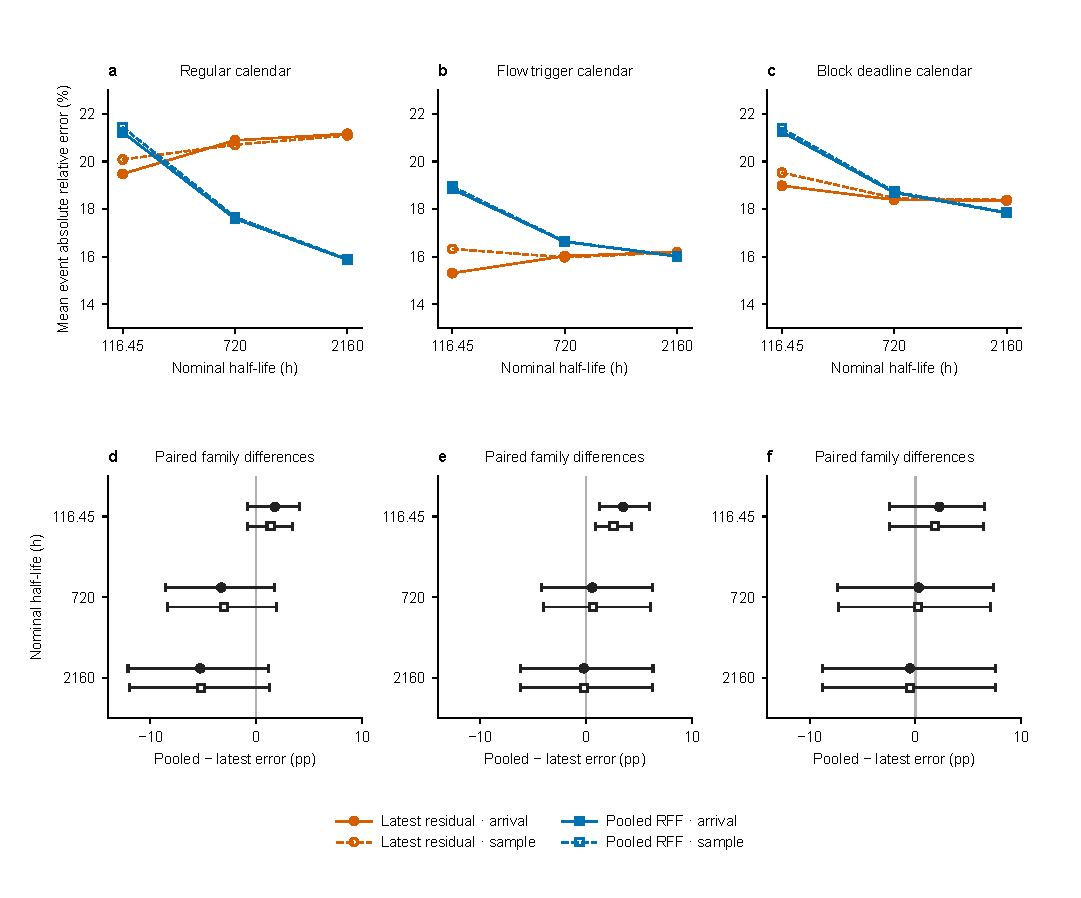
\includegraphics[width=\textwidth]{figures/Fig4.pdf}

\caption{Reconstruction family, nominal memory and age origin under fixed acquisition calendars. (a to c) All 36 development configurations: three sampling calendars, two reconstruction families, three nominal half lives and sample origin versus arrival origin ageing, with calendars held fixed at 96 attempted samples per year, an actual delay of 24 h and innovation feedback disabled ($\rho$ = 0). All points average the seven development sites after seed and year aggregation. Solid filled symbols mark arrival origin ageing and dashed open symbols mark sample origin ageing. (d to f) Paired mean error difference between pooled random Fourier features and latest residual reconstruction at the same calendar, nominal half life and age origin, with 95\% station bootstrap intervals, where circles mark arrival origin and open squares mark sample origin. Positive differences favour latest residual reconstruction. The 116.45 h nominal half life equals a 168 h exponential time constant. Matching a nominal half life does not match effective memory, because a latest residual estimator replaces its previous residual while the pooled estimator retains several contributions. These fixed calendar component comparisons do not evaluate a newly optimised sampling policy and they do not establish a universal ranking of reconstruction families.}
\label{fig:4}
\end{figure}

\subsection{Delay, pending information and quota fallback}

The main scenario with a 24 h real delay contains no earlier purchase that is still pending at an eligible acquisition decision. Queue correction is implemented and inactive under the 24 h minimum interval and the receive first ordering, so it cannot contribute to the reported main results. At a real delay of 72 h, pending purchases are present in 22,455 of 37,925 eligible candidates in the aware system traces with a maximum queue size of one, which activates the mechanism and allows its contribution to be tested (Fig. 5). The innovation scale sensitivity of the earlier experiment is a separate comparison that changes both query weighting and reconstruction weighting, and disabling adaptation there gives a temporal budget 96 value error of 26.53\% against 26.56\% with adaptation (Table F4; Online Resource 3).

Actual results arrive later than a sample taken at event onset would. At a temporal budget of 96 samples, the equal station mean fraction of event reference mass transported before the first usable arrival is 48.13\% for load value sampling and 46.97\% for flow triggering, and no usable result arrives within the event for an equal station mean 22.80\% and 18.27\% of events (Fig. S4). Those cases keep whatever information earlier results already supplied, so a missing arrival does not imply missing concentration information.

Holding the real delay fixed, the acquisition ablations leave mean error essentially unchanged (Fig. 5). At a true delay of 24 h and a budget of 96 samples, the immediate score alternative gives a mean event error of 16.71\% against 16.87\% for the delay aware rule, so the paired difference, alternative minus aware, is $-$0.16 percentage points with a station interval of $-$0.71 to 0.31 points. At a true delay of 72 h, the aware, immediate score and omitted pending errors are 22.12\%, 22.00\% and 22.03\%, and the paired differences, alternative minus aware, are $-$0.11 and $-$0.08 percentage points with station intervals of $-$0.43 to 0.26 and $-$0.40 to 0.30 points. The higher error at a real delay of 72 h therefore describes the complete system under a slower information clock with the specified updating rule. Because the residual correction used here decays from the arrival time, a longer real delay also changes the weight that the same residual carries at a given moment, so this cross delay comparison is not an isolated estimate of the effect of information lateness. A fixed calendar diagnostic separates the two (Table F5). With purchase timestamps held at the archived calendars at a budget of 96 samples, mean event error rose with the actual return delay under both decay origins: for flow triggered sampling from 14.4\% at 6 h to 17.7\% at 24 h and 23.1\% at 72 h with arrival origin decay, and from 14.7\% to 18.4\% and 23.3\% with collection origin decay. The paired difference, 72 h minus 6 h, was 8.67 points (station interval 5.15 to 12.72) for arrival origin and 8.66 points (4.62 to 12.98) for collection origin. Periodic and deadline sampling followed the same pattern, with paired 72 h minus 6 h differences between 5.20 and 6.53 points. Changing only the decay origin moved mean error by at most 0.92 points, and at 72 h the difference reversed sign for periodic sampling ($-$0.68 points, interval $-$2.83 to 1.62). The delay effect therefore persists under both definitions of residual age, while the origin of the decay is a small and uncertain choice on which the ranking of calendars does not depend. Because year end truncation removed only a small number of labels as the delay lengthened, this delay effect reflects when the correction becomes available and how much it has decayed rather than lost labels. Holding the calendars fixed also means that the 6 h and 72 h cells do not describe what those policies would have purchased at those delays, so the diagnostic measures the value of faster feedback under a given calendar rather than the full effect of changing the delay.

Raising the reference coverage requirement to 100\% changed the eligible set but not the conclusions (Table F6). The temporal cohort then contained eight stations and 29 events, with a load value error of 20.54\% against 20.67\% for flow triggering (paired difference 0.13 points, interval $-$1.35 to 1.48), and the additional stations contained six stations and 54 events, with 16.23\% against 17.83\% (paired difference 1.60 points, interval 0.37 to 2.89). Lowering the requirement to 90\% would add five temporal and four additional events without adding stations, but those events carry no scored endpoints in the archived results, so their paired differences cannot be computed; because the eligible sets are nested, the endpoints of the events common to both thresholds cannot change when the requirement is relaxed.

Quota fallback accounts for much of the calendar. Across all 13 data eligible temporal stations, load value deadline fractions rise from 60.26\% at a budget of 24 samples to 67.84\% at 48 and 76.44\% at 96, and flow fractions are 58.23\%, 65.97\% and 71.85\%. In the event primary subset the load value fractions are 52.16\%, 61.11\% and 70.52\%, and the additional station event primary fractions are 57.47\%, 73.61\% and 83.16\%. The direct deadline only comparison nevertheless shows that actively selected opportunities can matter, and keeping budget adherence separate from adaptive action prevents the first property from being read as evidence of the second. The complex rule also changed relatively few purchase times (Table F7). At a budget of 96 samples in the temporal cohort, load value and flow triggering shared 3127 of 3744 purchase timestamps and differed at 617, of which 217 fell within 6 h of each other; against periodic sampling they shared 36 timestamps and against pure deadline sampling 2879. Successful returns were similar across systems, with 3349 for load value against 3328 for flow triggering, 3329 for periodic and 3345 for deadline. A scoring rule can therefore act only inside the room that the quota, the minimum spacing and the deadline leave, and its contribution has to be read within those constraints. Station level differences show where updating helped and where it did not (Table F8): relative error improved at six of nine temporal stations and five of eight additional stations and worsened at three in each cohort, namely Grand River near Sumner (+3.17 points), Raccoon River at Van Meter (+2.05) and Embarras River at Lawrenceville (+1.91) in the temporal cohort, and Big Muddy River at Murphysboro (+8.05, with one eligible event among eighteen detected), South Raccoon River at Redfield (+0.32) and North Raccoon River near Sac City (+0.08) at the additional stations. Table F9 lists the 16 stations that enter the assessment cohorts, with their evaluation years, eligible events, median reference coverage, median peak flow, median reference concentration and historical residual persistence.

The isolated candidate diagnostic further bounds the interpretation of the load value score (Fig. S5). Of 168 fixed monthly candidates at seven development stations, 82 meet the declared spacing, label success and future window criteria. Adding the sample reduces absolute future window mass error for 50 candidates and increases it for 32, with a median relative reduction of 1.70 percentage points. The pooled rank correlation between acquisition score and kilogram error reduction is 0.153, and ranking both quantities within station gives 0.114. These weak descriptive associations leave the score as a proxy for realized utility rather than a calibrated measure of it, because the exercise holds subsequent purchases fixed and adds a sample instead of comparing two policies at an equal budget (Online Resource 1).

\begin{figure}[htbp]
\centering
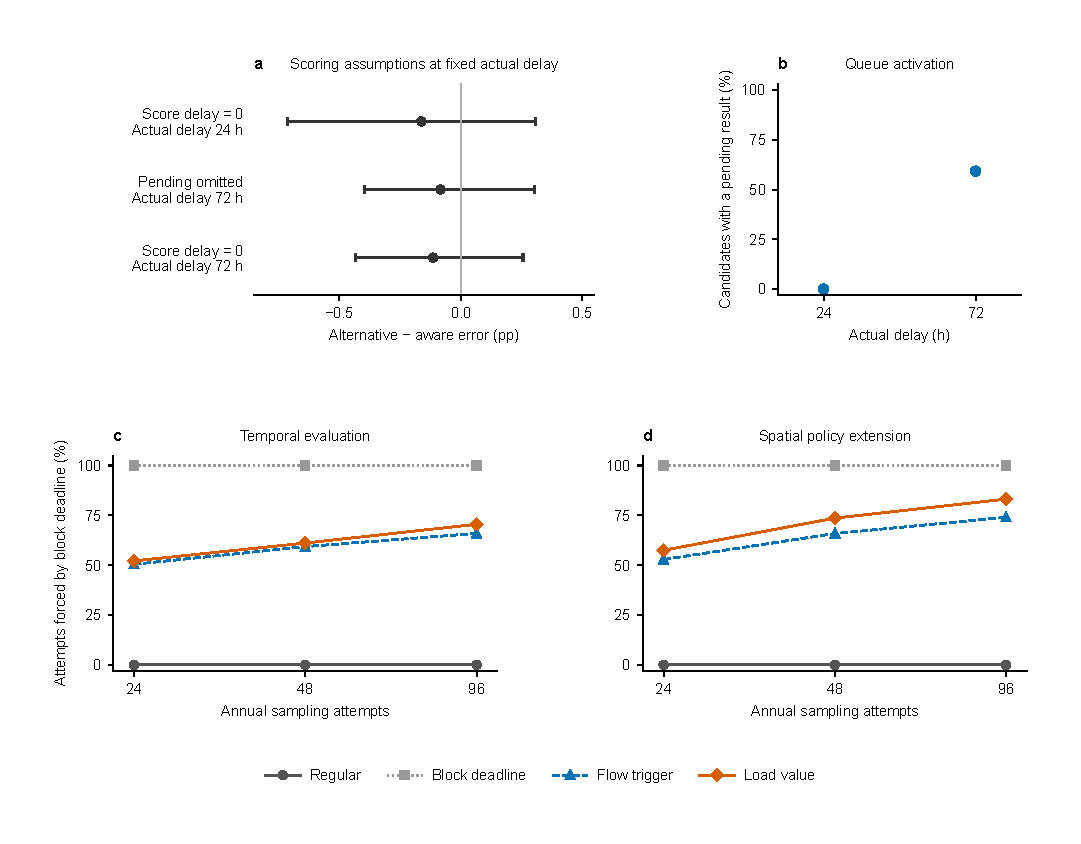
\includegraphics[width=\textwidth]{figures/Fig5.pdf}

\caption{Delay and pending result mechanisms are tested under fixed realized result return delay. (a) At 96 attempted samples per year, paired temporal station mean error differences between each altered scoring rule and delay aware, pending aware scoring, with 95\% station bootstrap intervals for the nine event eligible sites. The score delay zero variant still receives actual results after 24 or 72 h, and the pending omitted variant retains the actual 72 h delay. Positive differences favour the fully aware rule. These contrasts do not estimate a new effect of turnaround speed. (b) Fraction of eligible candidate evaluations with a result pending in the fully aware scenario: 0 of 38,019 at 24 h and 22,455 of 37,925 at 72 h, with at most one pending result. Candidate evaluations pool all 13 data eligible temporal sites and three seeds and they are an operational count rather than independent statistical replicates. At a 24 h delay the minimum 24 h spacing leaves the pending correction inactive at eligible candidates. (c, d) Mean station level fraction of attempts forced by block deadline fallback, restricted to each cohort event primary site set. Regular attempts are scheduled rather than forced, and the block deadline policy consists entirely of forced attempts. High fallback shares limit how much the adaptive score can change the acquisition calendar.}
\label{fig:5}
\end{figure}

\subsection{Process cases show both benefits and failures}

The three cases in Fig. 6 were selected from all 46 temporal events by the fixed rules of maximum improvement, maximum deterioration and nearest median for load value against flow triggering at a budget of 96 samples and seed 41. Both extremes occur at station 06902000 in neighbouring July events, and the rule output is reported without substituting a more favourable illustration.

For the event of 9 and 10 July, load value absolute relative error is 4.66\% against 41.92\% for flow triggering, and neither system received a usable result during the event. The difference therefore comes from the residual state left by observations collected before the event rather than from better event capture. In the event of 6 to 8 July, the load value system received its first usable event time result after 56.38\% of reference mass had been transported while flow triggering received one after 92.05\%, and yet load value error was 41.83\% against 13.79\% for flow. Its latest residual correction underestimated the transport that remained. At station 02035000 in the median difference event, collection and arrival times align and both systems have an error of 0.44\%. These cases connect realized chronology to estimator behaviour while the complete station display preserves the wider distribution, and they show that useful pre event state, early arrival and accurate correction are separate conditions.

\begin{figure}[htbp]
\centering
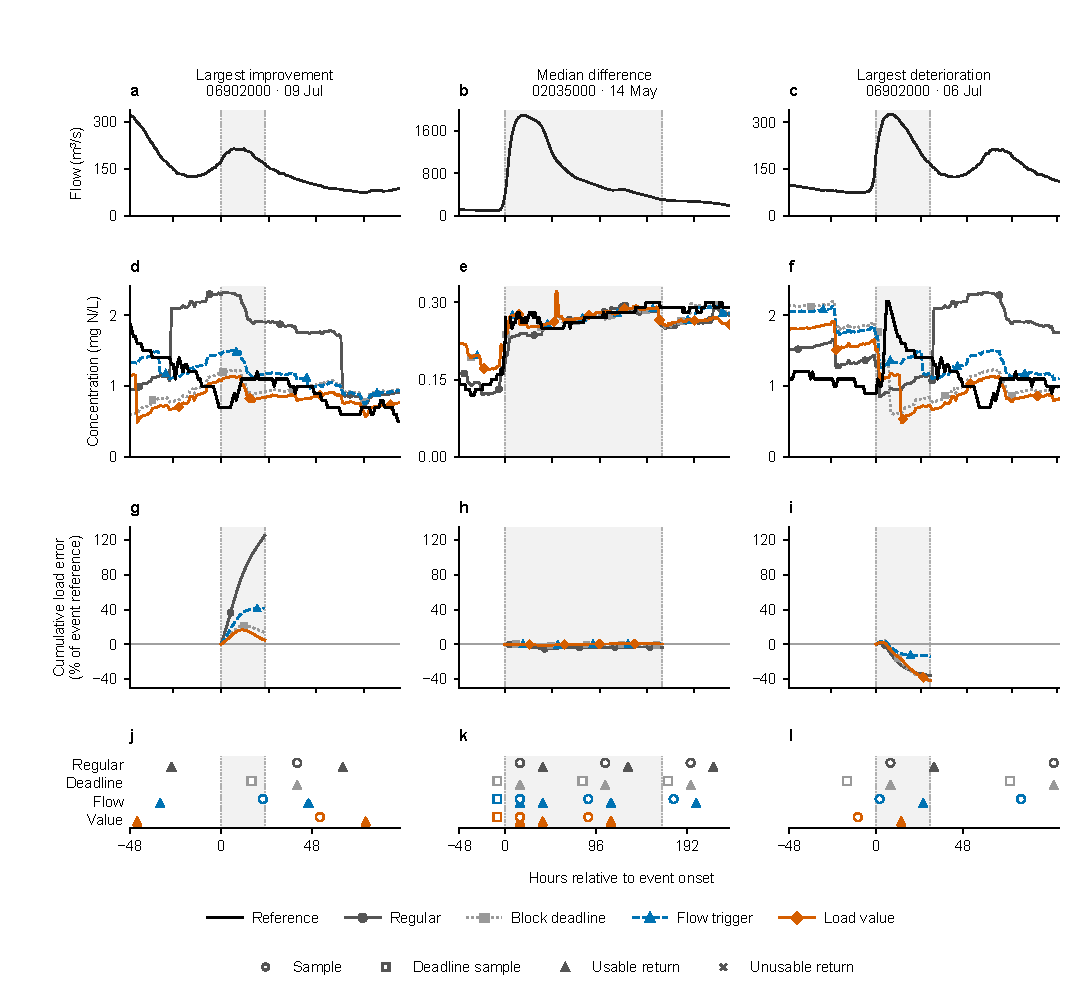
\includegraphics[width=\textwidth]{figures/Fig6.pdf}

\caption{Real event trajectories show improvement, a neutral difference and deterioration. Columns follow the largest improvement, the nearest median difference and the largest deterioration in load value versus flow trigger absolute relative error among the 46 retained temporal events at 96 attempted samples and seed 41. Selection is deterministic and illustrative, so these examples do not estimate a frequency of success or validate a mechanism. The two extreme cases occur at the same station in adjacent events and are reported without substitution. Rows show observed flow (a to c), exact hour reference concentration with four online concentration estimates (d to f), cumulative signed load error on common complete hour reference support (g to i), and independently aligned collection and return markers (j to l). Completed hourly mass integrals are plotted at the end of their hour and concentration estimates are plotted at issue time. Cumulative error is divided by the final observed event reference load rather than by a running denominator. Light shading marks each defined event, and curves can genuinely coincide. Samples are open circles, forced deadline samples open squares, usable returns filled triangles and unusable returns crosses, and samples and returns are separated vertically within each policy row only for legibility while their times are unchanged. Samples collected before event onset may return within the event. Predictions never use future returns and are never revised retrospectively, so return timing alone does not establish a benefit. The case records are observed support reconstructions rather than continuously complete river load truth.}
\label{fig:6}
\end{figure}

\section{Discussion}\label{sec:discussion}

\subsection{A returned sample must reach a useful estimator}

The strongest practical result in this assessment is the value of returned information relative to an unchanged historical model in the defined single year task. Two layers of improvement must be separated. At a temporal budget of 96 samples the systems that use returned samples reduce mean event relative error by about 14 percentage points relative to the historical predictor: the load value system by a paired mean of 14.87 percentage points, with every primary station improving, and flow triggered sampling by 14.0 points on the same endpoint. The second layer, the extra value of the complex rule over the simple hydrological trigger, is 0.83 points with substantial station variation and an interval that crosses zero, and the additional stations likewise do not establish a stable advantage over flow. For these records, improving the use of sparse returned results deserves attention before acquisition complexity is added, and the two layers should be reported separately rather than credited to the acquisition rule.

This finding develops an established monitoring insight rather than claiming that sampling and estimation are newly connected. Subsampling studies have shown competitive regular schedules and estimator dependent accuracy \citep{reynolds2016,lee2016,lee2019}, and residual aware load estimation already exploits temporal information beyond concentration and discharge regressions \citep{zhang2019}. The advance here is that these dependencies become evaluable under an explicit result return clock and an explicit provisional estimate clock, with a direct quota only competitor, complete systems that issue a credible simple correction, fixed calendar update diagnostics and fixed real delay acquisition tests. Those comparisons separate a sample that is collected from one that is returned, and a sample that is returned from one that improves the issued trajectory.

The two neighbouring events at station 06902000 show how much this separation matters. The largest benefit appeared without any result arriving during the event, and the largest harm appeared despite earlier arrival. Neither event capture nor early feedback is therefore a sufficient surrogate for estimation quality, and the direct evidence is the recorded state, the timing and the event error contrast. A plausible interpretation is that a recent residual can describe one segment of a changing concentration and discharge trajectory while failing on the next, and hydrological mixing and nutrient supply can alter that relationship during events \citep{bieroza2018}. The replay does not measure those sources or identify the biogeochemical mechanism, so the explanation remains a testable interpretation of the recorded behaviour.

\subsection{Memory, prior quality and the objective of acquisition}

Historical forward errors persisted over several days, which makes residual updating a reasonable choice, and persistence varied greatly across stations, which rules out a single correction lifetime. The fixed calendar factorial likewise does not support uniformly shorter memory: a long memory pooled updater performs well for some development calendars, including periodic sampling, while the latest correction holds an advantage in the short memory flow comparison. Pooling, shrinkage and residual age jointly determine how a returned sample changes an estimate, and equal numerical half lives do not produce equal responses because the two updating families forget different quantities. This is why replacing a weak shared updater can create a much larger apparent gain than changing the collection rule.

Predictor quality shifts the balance between benefit and risk. The additional station historical model starts from a lower mean event error of 19.07\% against 31.74\%, so less error remains to correct. At the largest budget the new corrections improve five of eight additional stations and deteriorate three, which is consistent with an update being risky when the historical estimate is already adequate and a single sparse residual represents a transient state. That pattern is a descriptive boundary of this record set rather than a fitted rule for disabling updates, and a prospective implementation could test historically calibrated update gates or state dependent persistence.

The acquisition objective introduces a further mismatch. The load value heuristic scores expected absolute residual load variance under its internal linear surrogate, while the primary evaluation weights event relative error equally, and large transports can dominate an absolute mass objective without dominating the relative error endpoint. The different mass error and relative error rankings in Table 3 illustrate the distinction, and the candidate diagnostic adds direct evidence that the surrogate score is only loosely aligned with realized absolute error reduction even within a fixed subsequent calendar. Its usefulness depends on covariance calibration, discharge persistence and agreement between the acquisition state and the output estimator. Separating the output rule from the acquisition state makes that dependence explicit instead of attributing to the score a value of information that belongs to the estimator.

An analyst therefore has to state the assessment objective before comparing policies, whether that objective is typical event relative accuracy, absolute transported mass or a stated operational tolerance, and the 10\% and 20\% summaries are examples of how the same results translate into an accuracy requirement. Any comparison of this kind benefits from keeping a credible simple schedule and a historical comparator in view, and a method that improves one endpoint while worsening another should be selected for its intended task rather than described as generally superior.

\subsection{What the delay and quota tests establish}

Real result delay matters for a provisional trajectory because information cannot change estimates that have already been released. The higher error of the 72 h system is compatible with the observed concentration of transport before arrival, and timing fractions remain descriptive because prior predictions, earlier observations and slowly varying residuals supply useful information in the meantime. Accounting for delay inside the score adds nothing measurable at a fixed real delay: pending information was absent from eligible decisions in the main scenario, and omitting it at 72 h left average error materially unchanged. These are informative mechanism limits rather than a defect of the implementation, and they define the conditions under which a different queue design could matter, namely decision intervals shorter than the return delay, sufficient overlap between outstanding samples, and acquisition opportunities that calendar obligations have not already exhausted. The tests cover the specified fixed delays with at most one pending purchase, and they do not represent arbitrary laboratory queues.

The high deadline fractions restrict claims of adaptive behaviour in the same way. The pure deadline baseline shows that avoiding some quota expiry purchases improves mean error, particularly at the largest budget, while the flow trigger captures much of that practical value from an observable hydrological signal. The evidence therefore supports a restrained engineering choice: compare extra complexity against its gain over flow triggered updating rather than against an unchanged prior alone. Nominal attempts and fixed delays make the comparison reproducible, and they are not estimates of transport, staffing, laboratory or maintenance savings.

\subsection{Scope and transfer}

The reference is a qualified optical nitrate plus nitrite record expressed as nitrogen. United States Geological Survey procedures and instrument specific safeguards improve traceability \citep{wagner2006,pellerin2013}, yet a sample and its evaluation reference can share sensor bias, fouling, optical interference or drift, and the assessment does not validate sparse laboratory measurements against this record. Adding independent Gaussian noise would not remove shared systematic error. The supported conclusion therefore concerns reconstruction of this sensor reference and its observed window transport, and independent chemistry together with real service records would be needed to extend it to laboratory accuracy and deployment reliability.

Missing reference intervals constrain the environmental interpretation further. Water volume coverage makes the support deficit visible, and the retained and excluded event diagnostics show that qualifying episodes are a selected subset of transport rather than a census. No observed concentration truth exists for excluded mass, so neither a full annual load nor a complete all event error can be recovered by relabelling the qualified window estimate. Reporting support alongside accuracy is therefore part of the result: a good conditional error over well observed intervals does not establish equivalent performance during sensor outages or poorly observed peaks.

The design also assumes an existing local high frequency baseline and simulates a single year of reduced concentration sampling with its own preceding historical window. It does not show that a station can operate sparsely for many consecutive years while its predictor remains current, and it does not show that an unmonitored river can adopt the policy without historical calibration. Historical hydrology can support sampling forecasts \citep{wilson2026}, while sustaining concentration prediction across several sparse years would require a sequential experiment in which unpurchased concentrations stay unavailable in every subsequent training year.

The geographical units remain limited to nine primary temporal stations in five HUC4 groups and eight additional stations in six groups. Station resampling, HUC4 deletion and the complete station displays characterise these records, and more hours, seeds or bootstrap draws do not enlarge the population of independent environments. All comparisons reported here were executed after the evaluation records had been inspected, so they describe these records and their mechanisms; confirming a selected modified system would require records that played no part in that process. Within those boundaries the assessment yields a practical monitoring contribution: it identifies which information is available at each decision, how that information changes the issued trajectory, and when added decision complexity earns a measurable benefit.

\section{Conclusions}\label{sec:conclusions}

Sparse concentration sampling adds most of its value to provisional river transport estimates when a returned result reaches a working estimator. In a single year reduction from a local high frequency nutrient record, returned sample updating with a single exponential residual correction reduced mean event relative error by 14.87 percentage points relative to an unchanged historical model and improved every temporal station, while flow triggered sampling improved the same endpoint by 14.0 points, so the gain belongs to the use of returned observations rather than to the complexity of the acquisition rule. The additional benefit of a load based trigger over a simple flow trigger was 0.83 percentage points with a station interval that includes zero, so the case for acquisition complexity rests on a margin that these records do not establish as stable. Fixed calendar diagnostics showed that updating family, memory and age origin can reorder sampler rankings, and fixed real delay tests showed that delay aware scoring and pending result correction leave mean error essentially unchanged when the underlying information clock is held constant. Monitoring programmes can therefore act on two findings that the records support directly, namely routing returned observations into the running estimate and stating the intended error objective before acquisition rules are compared; a third and more tentative direction is to choose the memory of that correction from the residual persistence observed at a station, which the fixed calendar diagnostics motivate without having tested it as a selection rule. These findings inform the choice of sampling and updating strategies for provisional nitrate plus nitrite load assessment at stations with an existing high frequency history. Their applicability is limited to qualified sensor reference windows, and they do not establish accuracy against independent laboratory measurements, complete annual loads or sustained operation over multiple sparse monitoring years.

\clearpage

\backmatter

\bmhead{Supplementary information}

Three Online Resources are provided as separate files with the submission: Online Resource 1 (supplementary methods and monitoring diagnostics), Online Resource 2 (complete comparison outcomes) and Online Resource 3 (earlier experiment settings, revision diagnostics and data provenance).

\section*{Declarations}

\begin{itemize}
\item \textbf{Funding} This research received no specific grant from any funding agency in the public, commercial or not for profit sectors.
\item \textbf{Competing interests} The author has no relevant financial or non financial interests to disclose.
\item \textbf{Ethics approval and consent to participate} The study analyses publicly available environmental monitoring records. It involves no human participants and no animal experiments, so ethical approval and informed consent are not applicable.
\item \textbf{Consent for publication} Not applicable.
\item \textbf{Data availability} Source observations and metadata are publicly accessible through the United States Geological Survey Water Data for the Nation service, using the station identifiers in Table S1, parameters 00060 and 99133, calendar years 2019 to 2025 and UTC timestamps; the archived subset was retrieved on 5 October 2026. The electronic supplementary material contains the hourly working data, metadata, exact query manifests, configurations, analysis code, complete comparison outputs, diagnostic selections and the source files for every table and figure, together with a README that lists the commands needed to reproduce each analysis. Access is through the electronic archive supplied with the manuscript, and no permanent public repository identifier is asserted. Subsequent live service revisions may differ from this archived snapshot.
\item \textbf{Materials availability} Not applicable.
\item \textbf{Code availability} The analysis code, the versioned hourly working data, the frozen configurations and every comparison output are supplied in the electronic supplementary material. The README in that archive lists the commands needed to reproduce each completed analysis.
\item \textbf{Author contribution} Junjie Zhang designed the study, prepared and quality screened the data, implemented and executed the chronological replay and the comparison analyses, interpreted the results and wrote the manuscript.
\item \textbf{Use of artificial intelligence} OpenAI Codex (a GPT-5 generation coding agent, OpenAI, accessed in October 2026) was used only for limited Python code assistance and English language polishing. All substantive research tasks, including study design, data collection and processing, analysis, interpretation, and manuscript preparation, were performed by the authors. AI did not generate or alter data or determine conclusions, and the authors take full responsibility for the manuscript. The tool supported code writing, debugging and refactoring for the replay and analysis scripts described in the Materials and methods and language editing in the Abstract, Introduction, Results and Discussion; every output was validated by rerunning the archived code against the recorded data and by comparing each table and figure value with its source result file, and all inputs are public monitoring records, so no sensitive, proprietary or human subject data were processed.
\end{itemize}

\bibliography{sn-bibliography}

\end{document}